%%%%%%%%%%%%%%%%%%%%%%%%%%%%%%%%%%%%%%%%%%%%%%%%%%%%%%%%%%%%%%
%%%%
%%%%  Project October
%%%%
%%%%%%%%%%%%%%%%%%%%%%%%%%%%%%%%%%%%%%%%%%%%%%%%%%%%%%%%%%%%%%
\documentclass[11pt,letterpaper]{article}
\usepackage[utf8]{inputenc}
\usepackage[letterpaper,includeheadfoot, top=0.5cm, bottom=3.0cm, right=2.0cm, left=2.0cm]{geometry}
\renewcommand{\familydefault}{\sfdefault}

\usepackage{graphicx}
\usepackage{color}
\usepackage{amsmath}
\usepackage{fancyhdr}
\usepackage{paralist}
\usepackage{hyperref}
\usepackage{subfig}
\usepackage{pdfpages}
\usepackage{amssymb}
\usepackage{url}
\usepackage{listings}

\usepackage{listings} %Code
\lstset{language=C, tabsize=4,framexleftmargin=5mm,breaklines=true}

\hypersetup{
    colorlinks,%
    citecolor=black,%
    filecolor=black,%
    linkcolor=black,%
    urlcolor=black
}

\begin{document}
%\begin{sf}

\newpage
\pagestyle{fancy}
\fancyhf{}
\fancyhead[L]{ 
\includegraphics[scale=0.3]{img/cwru-formal-logo-blue-no-tag.png} }
\vspace*{6cm}
\begin{center}
\Huge  {Project October}\\
\vspace{1cm}
\huge {Read news that you want to read}\\
\vspace{1cm}
\end{center}
%----------------- Names ------------------------
\vfill
\begin{flushright}
\begin{tabular}{ll}
Authors: & Tom Dooner, Mika Little, Brian Stack\\
Project: & Project October\\
Date: & \today
\end{tabular}
\end{flushright}

\newpage
\pagestyle{fancy}
\fancyhf{}

%\fancyhead[L]{\rightmark}
\fancyhead[L]{\small \rm \textit{\rightmark}}
\fancyhead[R]{\small \rm \textbf{\thepage}}


%\fancyfoot[L]{\small \rm \textit{Pie de página - Izquierda}}
%\fancyfoot[R]{\small \rm \textit{Pie de página - Derecha}}
%\fancyfoot[C]{\thepage} %Centro

\renewcommand{\sectionmark}[1]{\markright{\thesection.\ #1}}
\renewcommand{\headrulewidth}{0.5pt}
\renewcommand{\footrulewidth}{0.5pt}

% =============== Index ===============

\tableofcontents
\listoffigures

% =============== Section ===============
\newpage
\section{Abstract}

Longtime users of modern news aggregation services (such as Reddit, Slashdot, Digg, and Hacker News) report noticing a marked decrease in quality of discourse as the services gain mainstream attention.
This gradual, irreversible decline was noted as early as the newsgroup era, when new college students would log in for the first time in September, causing an influx of new users and subsequently diluting discussion upon the sites which they joined.
The situation worsened after AOL opened newsgroups to the masses, causing the community standards to continue to devolve, according to newsgroup veterans\cite{september}.
This gradual decline of content quality due to large numbers of new users came to be known as ``Eternal September'', being ``Eternal'' as the influx of new users was no longer restricted to September, but persisted through all months of the year. 
This phenomenon indicates that balancing a large community with high quality content is a challenge.

October is a solution to this problem.
By providing users with an automatically-customized experience, we believe we can provide a large community thoughtful discourse and interesting articles while avoiding the effects brought on by Eternal September.
October will employ a technique to recommend news articles which, to our knowledge, is not currently applied on any other major news aggregators.
With custom recommendations for each user, we believe that the October  community can attain large size without a sacrifice in quality.

\newpage

%----Everything else----%

\section{Project October: Hybrid Recommender System}

Due to the ever-growing amount of information available online, the need for a highly developed personalization and filtering system is growing significantly.
Recommender systems constitute a specific type of information filtering that
attempt to present items according the interests expressed by a user.
Most web recommenders are employed for e-commerce applications or customer
adapted websites, which assist users in decision making by providing
personalized information, but the same techniques that
suggest related items on e-commerce websites can recommend news articles to users as well.
We believe Project October is the first attempt to apply recommendation techniques to social news aggregation.

\subsection{Background}
It is our hypothesis that the recommendation of news sources will provide a scalable community experience that can be tailored to each person's interests.
Providing an automatic, customized, recommendation of articles will prevent the community from being diluted by new users and thus prevent the Eternal September phenomenon.
Each user will have their own viewing environment curated for them, with different mindsets and preferences forming their own communities in which like-minded individuals can partake in discussion, eliminating the cross-contamination of user bases.

%Brian! Come fill this background part out about the backend!

\subsection{Intended Audience}
Project October will be open to the public.
At launch, we will be inviting our friends from the CWRU community to try it out first, so we expect the user base to be somewhat technical in nature.

\subsection{Progress Since Progress Report 2}
% Fill in with details of our progress -- how far we have come and where we
% will go from here
Since Progress Report 2, we have implemented all our design requirements, released a beta version to the CWRU EECS department, and collected user metrics. More details about the v1.0 minimum viable product can be found in Section \ref{sec:release1.0}.

For the sake of releasing a minimum viable product within the semester, we have removed some complexity from our requirements in Progress Report 2. Specifically, we have made the following changes to the report, or the scope of our project:

\begin{itemize}
\item We have specified the plan for the backend recommendation engine in tangible terms.
\item We have removed the ability to upvote, downvote, and tag comments. Those abilities will be easy to add later but are not core to the application, especially until October gains critical mass and more people comment.
\item We have made numerous copy tweaks to the report, such as
  \begin{itemize}
  \item Reordering the report to list the requirements before the details of the project's implementation
  \item Adding Sections \ref{sec:frontendrss}-\ref{sec:tracking} about the frontend and Section \ref{sec:progress} about the overall final status.
  \item Moving the User Interface section into the requirements.
  \item Describing our testing process in Section \ref{sec:testing}
  \end{itemize}
\end{itemize}

\subsection{This Report}
% First we will describe the two separate components of October -- the frontend
% and then the backend. Then we will describe the API which ties them together.
% Then, we will discuss *how* we built October, including the requirements and
% the project management. etc.

\section{Software Design Requirements}
% This section will describe the progress towards the usual software design information, with likely components on
% - Application Software Requirements
% - Application Software Specifications
% - Software Architecture (i.e., client - server architecture; three - tiered design, etc.)
% - Design Document

\subsection{Homepage}
The are two cases for the homepage: logged in users and logged out users.

Logged out users arrive at the homepage and are presented with a splash page containing a description of October's features.
There is a registration link so that interested users can register for their own account.

Logged in users are, upon landing on the homepage, presented with a display of news articles.
Articles are displayed with pictures (when available) along with headlines.
Each article is accompanied with links to positively or negatively influence the article's recommendation rank, and also to comment on the article.
The source of the article is also provided, as is the time that it was posted.

\subsection{User Creation, Login, and Display}
New users are able to create October accounts with but three pieces of information --  their desired username, their email, and a password.
After creating an account, an email is sent to the user welcoming them to October.

When a user first logs into October, the backend recommender won't know anything about their interests.
Thus, users should be shown various sample topics to browse through.
They are also able to (via their account page) manually type in relevant keywords to aid the recommender in providing them with articles.

Every mention of a user's name (i.e. the credit for who posted an article or comment) is a link to a user profile page. More detail about the user profile page is given in Section \ref{sec:profilepage}.

\subsection{User Profile Page}
\label{sec:profilepage}
Each user has a profile page containing information related to that user.
The profile page contains a list of comments that the user has made on posts and a list of articles the user has posted.
All information on this page is public, as it is merely a summary of content available elsewhere on the public website.

\subsection{User Profile Edit Page}
In contrast to the profile page, which is a summary of a user's public activity, the profile edit page allows a logged in user to edit their own information.
Settings such as their email address and password can be changed here.

The other significant part of the user profile edit page is a section which shows the user their own recommendation settings.
This shows up in the format of a list of keywords that the backend has ascribed to that user.
The user can remove keywords that they do not wish to be associated with.

Furthermore, there should be a field where a user can submit additional keywords they wish to see more news from.
The user will be associated with the keyword when they submit the form.

\subsection{Article Posting}
Logged in users are able to click a link on the homepage to submit a story.
The submit story page will ask for the link to the desired story, and automatically show the results of scraping that story's contents (see Section \ref{sec:scraping} for more about scraping).
If the post looks good to the user, he or she can click a ``Post!'' button, which will persist the news story in all appropriate databases.

\subsection{Article Display Page}
The article display page is a page dedicated to a posted news article. Every news article has an associated article page.
The intent of the article page is to facilitate sharing of opinions around the posted news story through comments.

A user arriving on an article's page arrives at a page which contains the title of the news article along with a threaded comment list.
Users may leave comments as children of other comments, and thus may engage in a lively discussion.

\subsection{Frontend $\leftrightarrow$ Backend API}
Since the frontend and backend are divided with a Service Oriented Architecture (with Apache Thrift bridging the gap\footnote{See Section \ref{sec:api} for more about Thrift}), there must be an API between them.

The API should be as simple as possible to maintain the functionality of October. This is not a public API, so it needs to be robust to volume but we do not need to implement API endpoints for the functionality mentioned elsewhere in the requirements.

The API is defined in a Thrift definitions file in the project-october-api repository on GitHub\cite{project-october-api}.

\subsection{Backend} % Expand into multiple sections?
The backend is a recommender black-box which provides suggestions via an API to the frontend.
The actual implementation of the recommendation service is arbitrary, only that it implements the services of the API effectively.
For more about the implementation of the backend, consult Section \ref{sec:backend-implementation}.

\section{Application Architecture}
\subsection{Frontend}
The frontend is similar in function to a standard social news aggregator.
Upon going to the homepage, new and logged-out users are presented with a splash page that describes the nature of Project October and are given a registration link.
Users can register for the application by selecting a username and password.
A registration confirmation is emailed to newly registered users.

When logged in, users are presented with their personalized content.
The design is modelled after the front page of a newspaper -- articles that are evaluated to be more interesting to a user are placed in more prominent positions while articles that are deemed less relevant to the user's interest will fill the side columns, be located further down the page, and occupy less space.
Users are able to click on the headline (or associated image, if existent) to be taken to the original news source.

Each news article features a link to view the associated comments as well as icons which allow the user to plus and minus the article.
These are analogous to upvoting in Reddit, except that plusing or minusing an article on October will inform the recommendation engine of your individual preference, rather than directly impacting the weighting of an article by a predefined formula.
Therefore, voting serves two purposes: to inform other users of the quality of the article and to inform the recommender system of the user's interests.

Users will be able to click a link on the homepage which takes them to an article submission form.
The submission form requests a URL and a headline for that news story.
Upon entering the URL, the news story is scraped in the background using a web scraping tool which attempts to extract properties about the page automatically -- relying upon the <meta> tags and heuristics to determine the article's body text. The user is also presented with a list of tags that are garnered from the article, and they can delete or add their own tags to better represent the content of the article. A list of scraped images is also presented, and the user may select which one (if any) they want to head the article with. 

\subsubsection{RSS Subscription}
\label{sec:frontendrss}
% we added the ability to subscribe to rss feeds. this is a cheap way to find more news articles but it also helps us get users who are longing for a replacement for google reader.

\subsubsection{Article Layout Algorithm}
% right now the layout algorithm is pretty basic. Receiving a list of weights, pick the top two with pictures and make them "featured" articles.
% The next highest-weighted 50% of articles are displayed at a primary size and the rest are displayed in a secondary size.
% Then, articles are shuffled slightly and displayed to users

\subsubsection{Article Display Sizes}
% articles can be in three sizes -- featured, primary, and secondary
% primary and secondary can be either with image or without image

\subsubsection{Backend Proxy}
% a proxy exists which will keep the frontend functional in case of problems with the backend.
% It is a Ruby wrapper around the thrift library which will automatically retry an API call upon failing the first time (in case of disconnect) and will switch to the Mock Backend in case of total failure.
% In that state, October is operating without its brain, so users are presented with a vibrant message

\subsubsection{Sending Email to Users}
October uses Ruby on Rails's packaged ActionMailer to send emails.
We use the premailer Ruby gem to speed up development -- it allows for the use of real stylesheets which are then compiled inline to the appropriate HTML elements of the emails before they are sent.

Currently, the only email that is delived is a welcome email for the user offering basic onboarding instructions.
However, in the future, we intend to engage users via email with customized recommendation emails (i.e. ``We just found this article that we know you will like!'')

\subsubsection{User Tracking + Analysis}
\label{sec:tracking}
In order to understand how effective our users find October, we have instrumented the site with a heavy dosage of analytics.
To track basic page views and real time events, we have installed Google Analytics.
But, Google Analytics does not provide the granularity that we would need to adequately understand user behavior.
To this end, we have instrumented the site with Mixpanel\cite{mixpanel}, which specializes in tracking user-triggered \textit{events} rather than simple pageviews.

Mixpanel helps us track user behavior by tracking an event every time a user performs one of the following actions: log in, sign up, receive recommendations, vote, click article headline, or post a new article.

We currently use Mixpanel is a couple ways beyond simply tracking user events, however. Primarily, we track how many milliseconds the user waits to receive recommendations from the backend.
We also track the direction of users' votes, so we can tell how satisfied users are, at a high level, with their article recommendations.

\subsection{Web Scraping}
\label{sec:scraping}
We use a library called Pismo~\cite{pismo} to scrape
webpages.  While this may seem like a trivial operation that we should implement
ourselves, there is much that must be done in order to determine the actual
content of a webpage.  We have selected to use the "cluster" approach Pismo
provides to determine which parts of the webpage are actually content.  This
approach ranks each $<$div$>$ element on a page according to the following
heuristics:

\begin{enumerate}
 \item element must contain text
 \item earlier elements are more likely to be in the body of text
 \item each element must be over some minimum length (80 characters by default)
 \item more text in an element and more "." delimited sentences raise chance of
being content
\end{enumerate}

This works well for our purposes.  It is possible that as time progresses, we
can make use of HTML5 semantic tags such as $<$article$>$ in order to more
accurately extract text.

Once this text is extracted, Pismo relies upon the
Phrasie~\cite{phrasie} library to determine keyword tokens.
The initial version of Pismo we used was based upon a naive list of (token,
freqency) pairs, however Phrasie uses parts-of-speech to determine keywords and
gives them a weight rather than a straight frequency.  The strength of this
approach is that it results in a much higher signal-to-noise ratio than the
naive approach.  A weakness is that we've now reduced our possible languages
down to just english.  As time goes on we can modify this approach to either
support more languages or just work in a general sense on any language.

We also make use of Pismo's ability to extract images on the page that have a
high likelihood of being content rather than UI elements.

Firgure \ref{fig:nytimes} gives a visual representation of the content on a page
we want to scrape.

\begin{figure}
\centering
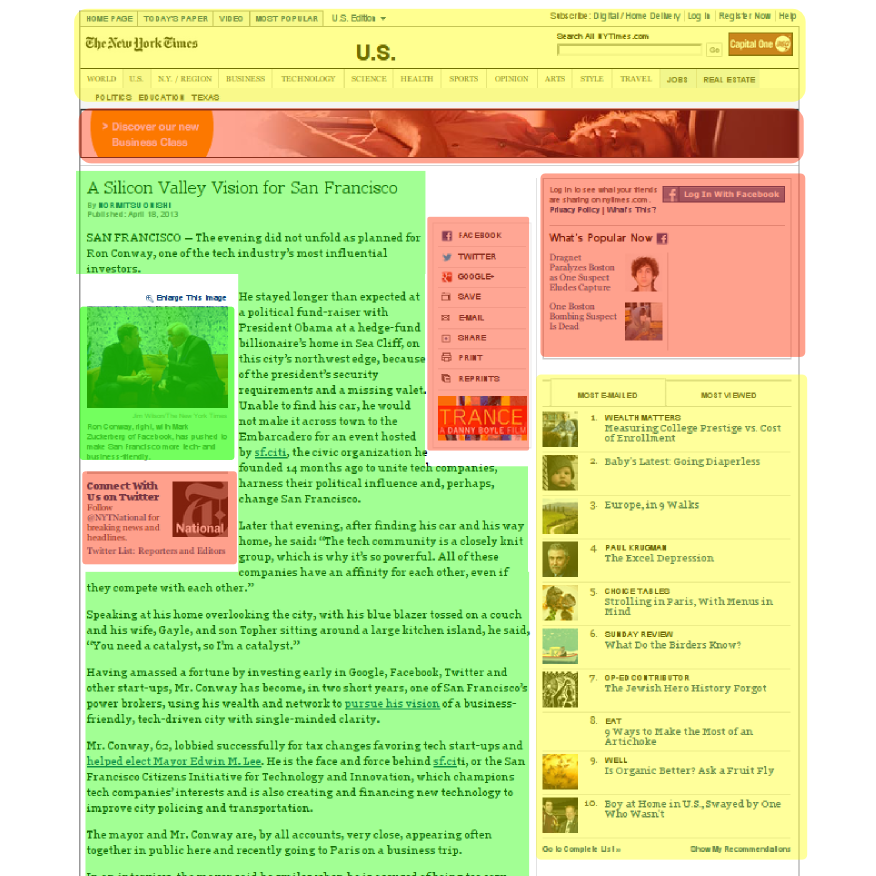
\includegraphics[scale=0.5]{img/nytimes.png}
\captionsetup{singlelinecheck=off}
\caption[foo]{\begin{small}Sections of webpage colored by desirability. \begin{description}
 \item[Green] Sections are best for determining content of article. Also
  includes potential images to use as a headline image for the article.
 \item[Yellow] Sections may contain useful information but are not part of the
  body of the article.
 \item[Red] Sections do not contain useful information and will harm results if
  included.
\end{description}\end{small}}
\label{fig:nytimes}
\end{figure}

\subsection{Backend}
\label{sec:backend-implementation}
\subsubsection{Vectorization of Posts}
The scraper from section \ref{sec:scraping}
\subsubsection{Vectorization of Users}
\subsubsection{Tf-Idf}
\subsubsection{Signals}
\subsubsection{Time Scaling}

\subsection{Frontend/Backend API}
\label{sec:api}
October will employ an API to promote separation between the frontend and the backend recommender system.
This will provide a clear interface and facilitate easy simultaneous development of both parts of October.

To implement the API, we will use Apache Thrift, an Interface Description Language\cite{thrift}.
The essence of the API is simple, featuring primarily two types of calls:
\begin{description}
\item[Give $n$ recommendations for user $u$]
This is the main output from the backend, returning recommended news stories or comments for a given user.
Ancillary parameters will be added to this to facilitate the frontend placement of articles, e.g. the recommendation confidence and individual article weightings.
\item[User $u$ took action $n$]
This is the main input to the backend, allowing it to adjust recommendations according to user action.
The parameters to this API call can be of many types. For example, "User commented on article \#$n$", "User gave cred to comment \#$n$", and "User visited link \#$n$" are all valid parameters for this API call.
\end{description}

These two calls manifest themselves in Thrift with a few simple object
definitions and an interface.  The abbreviated version \texttt{0.1.0} is
attached as Appendix~\ref{app:thrift}.

\section{Project Management--Administrative Details}
% Design/update your Gantt chart to show any changes in milestones, timetable,
% or responsibility (especially if there are multiple team members). Be sure to
% properly indicate who is actually performing each task and the degree of
% completion of each task.  Describe how well the project management plan is
% working. Were there unforeseen problems with any of the tasks that you ha ve
% had to work around? Are there delays in obtaining parts or software?  Were
% major changes to the management plan or back - up plans requ ired and
% implemented? What work - arounds were necessary to keep the project on
% schedule?  It is very important that you des cribe any changes in the project
% plan since the proposal and the reasons for them.  Finally, use your
% management plan to carefully think about what can be realistically done by
% your 3 team between now and the end of the semester.

\begin{figure}
\centering
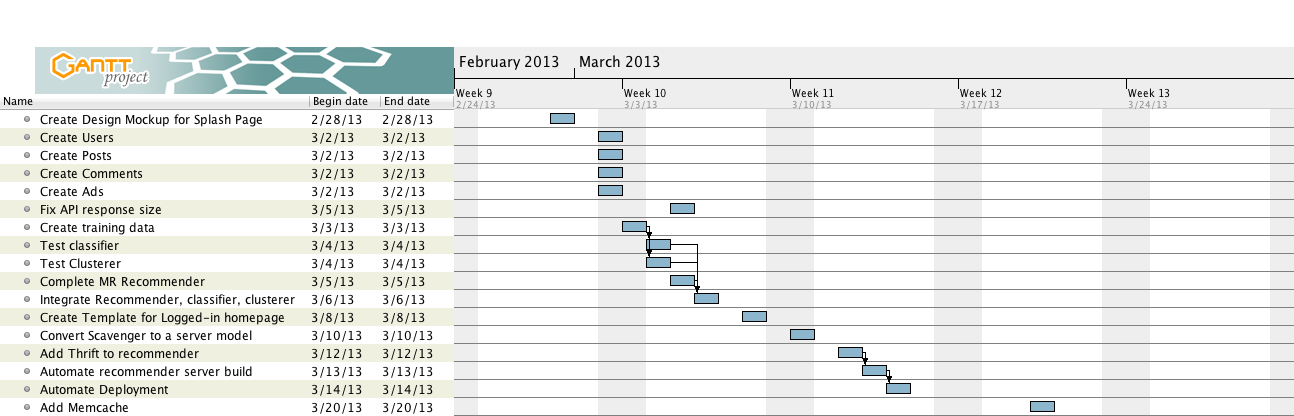
\includegraphics[scale=0.45]{img/octoborg-gantt.png}
\caption{Project October Gantt Chart}
\label{fig:gantt}
\end{figure}

We have split the team into two parts, frontend and backend.
With respect to the frontend, Tom and Mika have worked on the development and design respectively.
The biggest difficulty here is to determine how to represent the news in such a way that the user will be inclined to continue using the service.
As for the backend, Brian has been tasked with creating both the service architecture and the recommender engine.
This includes the implementation of our backend's TF-IDF algorithm and the Scala connector to the Thrift API and Mongo that computes recommendations.

\subsection{Release v1.0}
\label{sec:release1.0}
In Project Report 2, we promised a fully-functional beta by ``early to mid-April''.
On April 15th, we released the beta to the CWRU community, and it has been met with a warm reception.

\section{User Interface}
The user interface for the homepage and other pages will surely evolve over time.

The homepage is an especially crucial interface to get right. We mimic a newspaper feel with articles staggered in a rough column grid.
This allows readers to be presented with many recommendations of different weights simultaneously in a manner in which they are accustomed to. 
Cred will be handled by placing two links (upvote and downvote) into the article area, along with the link to the comments next to it. 
The search bar, along with a 'Submit Article' button, and Profile drop-down menu will be located at the top of the site. The latter will include options such as "view posts", "Profile Edit", "New Messages/Comments" and "Logout".
The comments on each article are handled in a nested fashion, with each comment and reply having their own attributed cred value. 
% TODO: Make sure we change this line/section as we go through the project:
A pre-Alpha screenshot of the homepage is attached in figure \ref{fig:homepage}.

\begin{figure}
\centering
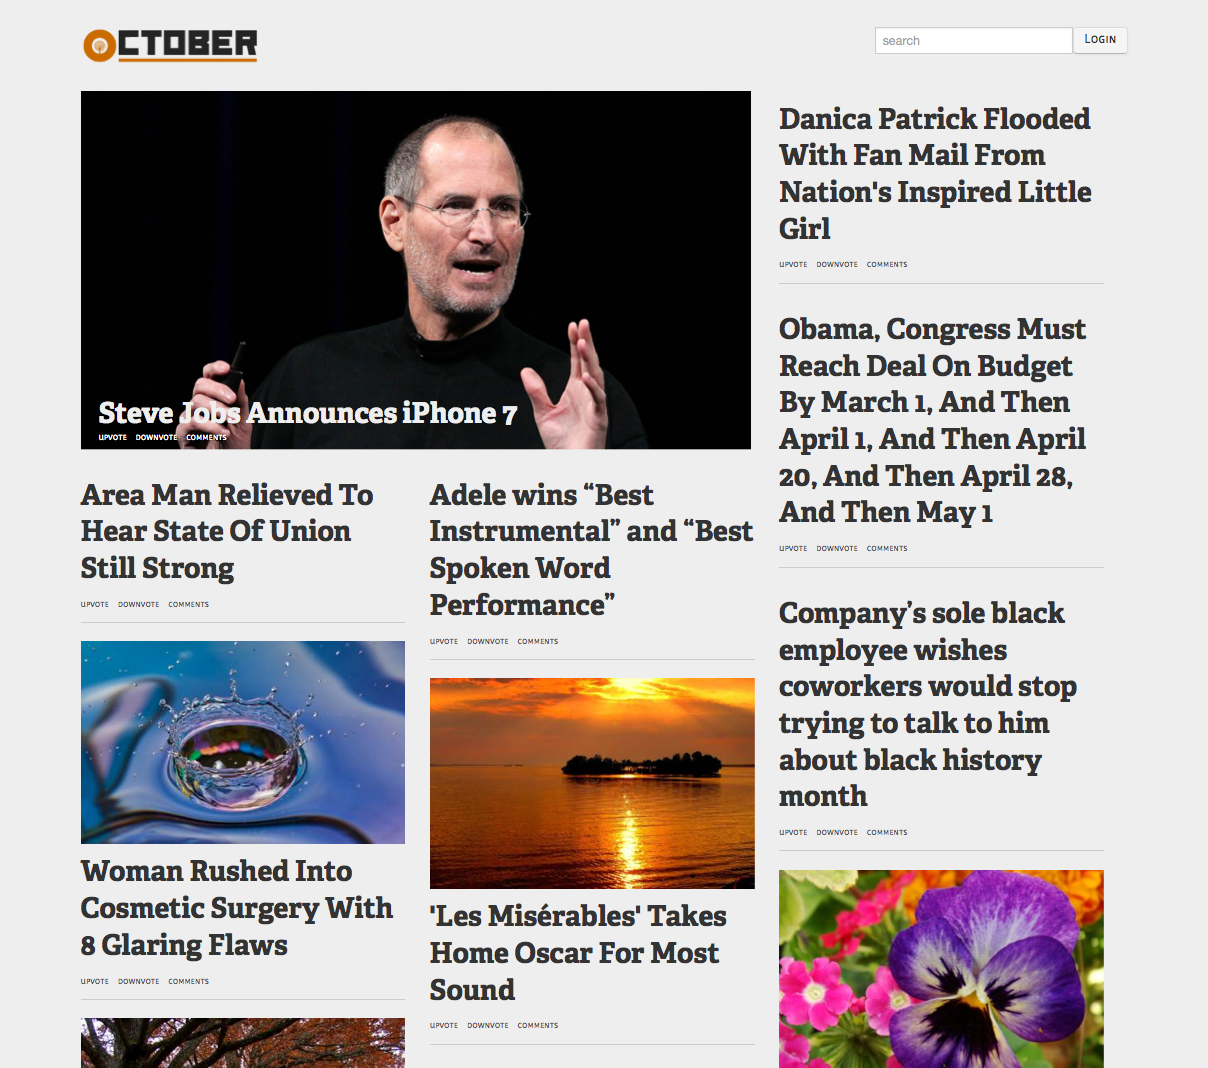
\includegraphics[scale=0.35]{img/homepage.png}
\caption{Project October Homepage, pre-Alpha (Headlines courtesy The Onion)}
\label{fig:homepage}
\end{figure}

The user interface for other pages will be in the same general content area, however there are no further screenshots to share at this time.

\section{Testing \& Evaluation}
\label{sec:testing}
Testing and evaluation will be performed as we progress through the project. Currently, only very minimal testing is implemented.

\section{Project Progress}
\label{sec:progress}
% This section should summarize the progress (or the lack of it) so far, and
% address any issues that have arisen recently.
The project is progressing satisfactorily.
We are attempting to follow Agile Design Patterns, and we have been effective at meeting for short periods frequently.
On the frontend, we have completed the user creation + login processes, mocked up the homepage, and connected the Thrift library.
On the backend, we have implemented the API so it responds to requests from the frontend. The recommendation engine is still in-progress.
We remain committed to maintaining team communication via scrum and continue working.

\subsection{Discussions \& Conclusions}
% These conclusions are not really conclusions since your project is not yet
% finished. In this section you should discuss whether the project is on
% schedule for completion at the end of the semester. Are there major problems
% which require a reevaluation of the project results? If not, what is the new
% schedule and what do you plan to have done by the end of the semester? You
% can also comment on things which have worked better than expected or proved
% easier to solve.
Overall, the project is still on schedule. We still intend to complete a fully-featured product on-time.

\section{Lessons Learned}

%The lessons we've gleaned through development. If you've had any personal %revelations, visions, or epiphanies, please share below. 
Throughout the development of October, we gained insight as how to properly design and create a product that will be used by many. 
Foremost among lessons learned, is that agile development ended up not being suitable for our work agenda. 
It required a certain rigidness in our schedules that we could not maintain. 
Instead, periodic scrum meetings sufficed for communicating progress and sharing ideas. 

Alongside the ineffectiveness of agile development in a college setting, an important lesson was learned when October was first released to the public in early April. 
Based on user feedback, we learned that October was, in fact, a viable web service, and we have had moderate user retention. 
We have enjoyed working on this, and we hope to continue refining it after the class is over. 
We will be keeping in contact with users to build upon October, enhancing the service and hopefully increasing user retention.

\subsection{Advantages \& Disadvantages of a Service Oriented Architecture}

\section{Appendix}

% ============= References ==============
\newpage
\newpage
\begin{thebibliography}{6}
  \bibitem{september} \url{http://en.wikipedia.org/wiki/Eternal\_September}
  \bibitem{thrift} \url{http://en.wikipedia.org/wiki/Apache\_Thrift}
  \bibitem{tfidf} \url{http://en.wikipedia.org/wiki/Tf-idf}
  \bibitem{pismo} \url{https://github.com/peterc/pismo}
  \bibitem{phrasie} \url{https://github.com/ashleyw/phrasie}
  \bibitem{mixpanel} \url{http://mixpanel.com}
  \bibitem{project-october-api} \url{https://github.com/bis12/project-october-api}
\end{thebibliography}

% ============= Database Schematic ==============
\newpage
\appendix
\section{Thrift API Definition}
\label{app:thrift}
\begin{verbatim}
const string VERSION = "1.0.0"
struct Post {
    1: required i64 post_id,
    2: optional double weight,
}
struct PostList {
    1: optional double confidence,
    2: required list<Post> posts,
}
struct User {
    1: required i64 user_id,
}
struct Token {
    1: required string t,
    2: required i32 f,
}
enum Action {
    READ,
    VOTE_UP,
    VOTE_DOWN,
    VOTE_UP_NEGATE,
    VOTE_DOWN_NEGATE,
    POST,
    COMMENT,
    REPORT,
    TAG,
    FOLLOW,
}
service Recommender {
    string ping() throws (1: TimeoutException te),
    PostList recPosts(1: required i64 user_id, 2: required i32 limit, 3: required i32 skip)
      throws (1: NotFoundException nfe, 2: EngineException ee, 3: TimeoutException te),
    bool addUser(1: required i64 user_id)
      throws (1: EngineException ee, 2: TimeoutException te),
    bool addPost(1: required i64 user_id, 2: required i64 post_id, 3: required list<Token> raw_freq)
      throws (1: EngineException ee, 2: TimeoutException te, 3: NotFoundException nfe),
    bool userToPost(1: required i64 user_id, 2: required Action verb, 3: required i64 post_id)
      throws (1: NotFoundException nfe),
    bool userToComment(1: required i64 user_id, 2: required Action verb, 3: required i64 comment_id)
      throws (1: NotFoundException nfe),
    bool userToUser(1: required i64 actioner_id, 2: required Action verb, 3: required i64 actionee_id)
      throws (1: NotFoundException nfe),
    map<string, i64> userTopTerms(1: required i64 user_id, 2: required i32 limit)
      throws (1: NotFoundException nfe),
    map<i64, double> textSearch(1: required list<string> tokens, 2: required i32 limit, 3: required i32 skip)
      throws (1: EngineException ee),
    bool addUserTerms(1: required i64 user_id, 2: required list<string> terms)
      throws (1: NotFoundException nfe),
    bool removeUserTerms(1: required i64 user_id, 2: required list<string> terms)
      throws (1: NotFoundException nfe),
}
\end{verbatim}

\section{Database Design}
\subsection{Frontend Database}
\begin{figure}
\centering
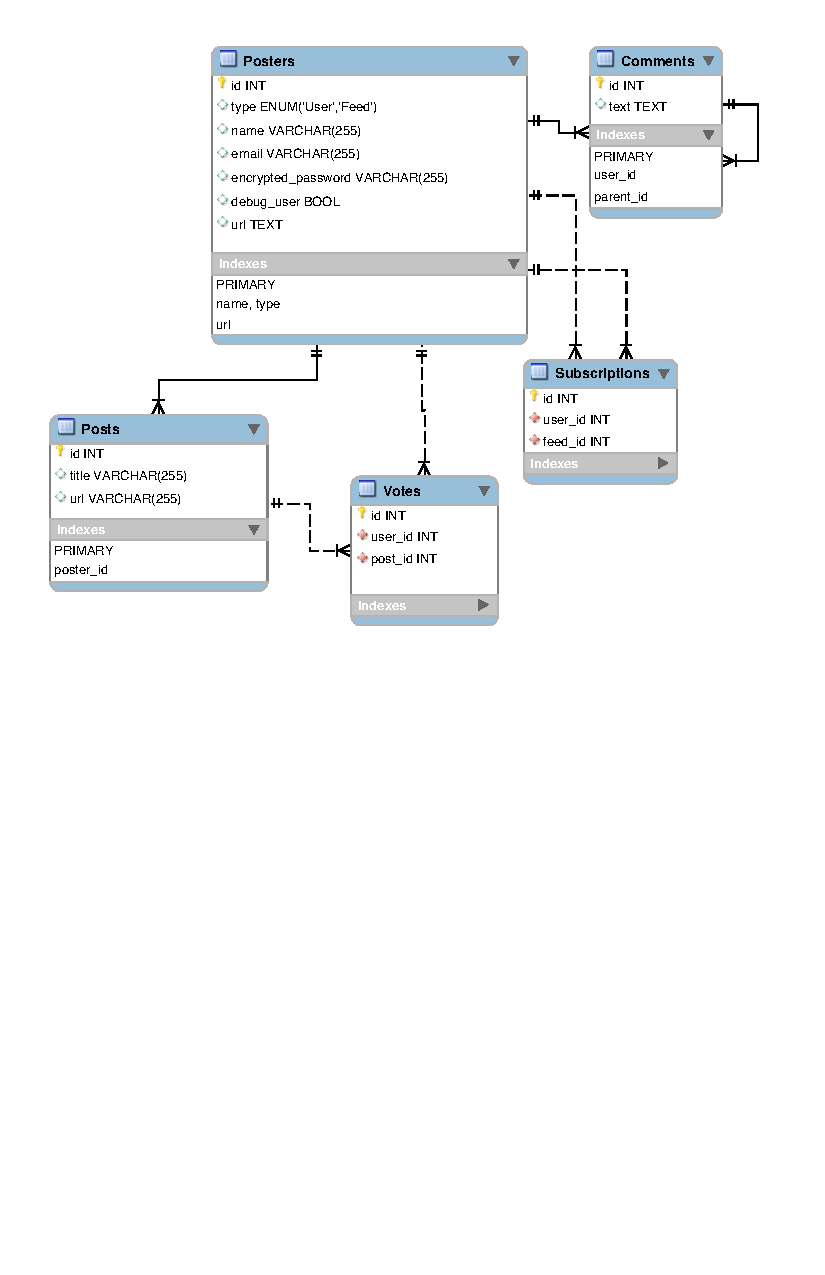
\includegraphics{db_diagram.pdf}
\caption{Frontend Database Relational Diagram}
\label{fig:database}
\end{figure}
Please see Figure \ref{fig:database}.
\subsection{Backend Database}

\section{User Manual}

\section{Programmers Manual}
% ============= FIN ==============

\end{document}
